%%%%%%%%%%%%%%%%%%%%%%%%%%%%%%%%%%%%%%%%%%%%%%%%%%%
%% Modèle de rapport pour l'application BI
%% Vincent Labatut 2014-21 <vincent.labatut@univ-avignon.fr>
%%%%%%%%%%%%%%%%%%%%%%%%%%%%%%%%%%%%%%%%%%%%%%%%%%%
%% Classe du document
\documentclass{ceri/sty/rapport}
% \documentclass[handout]{ceri/sty/rapport}
% \documentclass[light]{ceri/sty/rapport}
% \documentclass[full]{ceri/sty/rapport}
% \documentclass[blue]{ceri/sty/rapport}

%%%%%%%%%%%%%%%%%%%%%%%%%%%%%%%%%%%%%%%%%%%%%%%%%%%
\major{Master 2 informatique}
\specialization{ILSEN/IA}
\course{Business intelligence \& Systèmes décisionnels}
\subcourse{Application Business Intelligence}
\title{Démissions d’un organisme bancaire}

%TODO Liste des auteurs
\author{
	Prénom1 Nom1 \\ % il faut aller à la ligne entre chaque auteur
	Prénom2 Nom2 \\
	Prénom3 Nom3
}

\advisor[Responsable]{
    Vincent Labatut
}

%TODO Groupe des auteurs
\group{Groupe xx}

% Date de finalisation du rapport. 
% La valeur par défaut, qui est recommandée, est la date du jour.
%\date{\today}

%%%%%%%%%%%%%%%%%%%%%%%%%%%%%%%%%%%%%%%%%%%%%%%%%%%
% Désigne le fichier bibliographique à utiliser
\addbibresource{bibliographie.bib}

%%%%%%%%%%%%%%%%%%%%%%%%%%%%%%%%%%%%%%%%%%%%%%%%%%%
\begin{document} 

% Création de la page de titre.
\maketitle

% Justification moins stricte : empêche certains mots de dépasser dans la marge
\sloppy      













%%%%%%%%%%%%%%%%%%%%%%%%%%%%%%%%%%%%%%%%%%%%%%%%%%%
%%%%%%%%%%%%%%%%%%%%%%%%%%%%%%%%%%%%%%%%%%%%%%%%%%%
\section{Présentation}

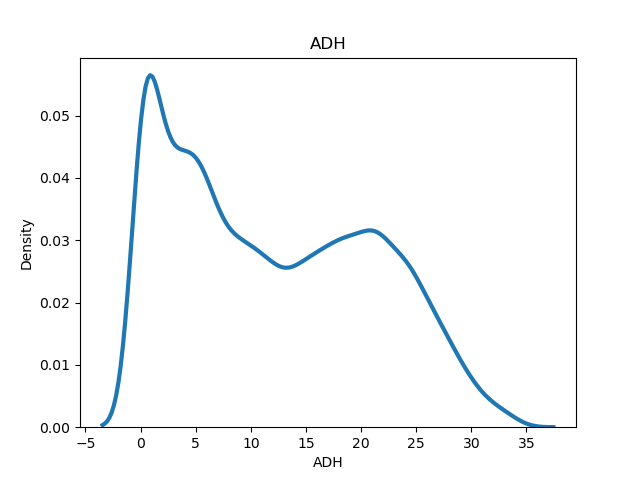
\includegraphics{fig/ADH}

Si vous utilisez \LaTeX{} pour écrire votre rapport, veuillez consulter le tutoriel fourni à l'adresse suivante : \url{https://www.overleaf.com/latex/templates/modele-rapport-uapv/pdbgdpzsgwrt}. Attention, il vous faut accéder au \textit{code source} pour bénéficier des commentaires qu'il contient, et qui complètent le texte apparaissant dans le PDF produit.

Le reste du document présent décrit la structure imposée pour votre rapport. Vous devez obligatoirement la suivre, en respectant les titres et la numérotation indiquée. Les listes de points à l'intérieur des sections sont là pour décrire le contenu que vous devez produire. \textbf{Ne reprenez pas ces points \textit{verbatim} : il s'agit simplement d'indications.}

\begin{beware}[Remarque]
Si vous faites une copie de ce document, configurez Overleaf pour qu'il le compile avec \href{https://fr.wikipedia.org/wiki/LuaTeX}{LuaLaTeX}. De plus, vérifiez que le correcteur orthographique sélectionné est bien celui destiné au français.
\end{beware}




%%%%%%%%%%%%%%%%%%%%%%%%%%%%%%%%%%%%%%%%%%%%%%%%%%%
\subsection{Contexte}
\begin{itemize}
	\item Rappelez brièvement le contexte du projet et ses objectifs.
\end{itemize}




%%%%%%%%%%%%%%%%%%%%%%%%%%%%%%%%%%%%%%%%%%%%%%%%%%%
\subsection{Organisation}
\begin{itemize}
	\item Décrivez la composition du groupe, la répartition du travail.
	\item Indiquez comment votre travail a été organisé dans le temps.
	\item Indiquez aussi comment les tâches ont été distribuées entre les membres du groupe (qui a fait quoi ?). Il s'agit de décrire les tâches \textbf{individuelles}, donc vous devez les décomposer à un niveau suffisamment détaillé pour permettre de décrire ce que chaque membre du groupe a fait.
	\item Indiquez quelles bibliothèques vous avez utilisées, en expliquant leur rôle. S'il s'agit de bibliothèques différentes de celles utilisées en TP, \textbf{expliquez} la raison de votre choix.
\end{itemize}



















%%%%%%%%%%%%%%%%%%%%%%%%%%%%%%%%%%%%%%%%%%%%%%%%%%%
%%%%%%%%%%%%%%%%%%%%%%%%%%%%%%%%%%%%%%%%%%%%%%%%%%%
\section{Données}

%%%%%%%%%%%%%%%%%%%%%%%%%%%%%%%%%%%%%%%%%%%%%%%%%%%
\subsection{Caractéristiques}
\begin{itemize}
	\item Décrivez les données et l'exploration que vous en avez faite.
	\item Soyez exhaustifs : fichiers de données, liste des attributs, nature et codage des valeurs, interprétation, unité dans laquelle la variable est exprimée (pour les variables numériques), etc.
\end{itemize}




%%%%%%%%%%%%%%%%%%%%%%%%%%%%%%%%%%%%%%%%%%%%%%%%%%%
%\subsection{Nettoyage et fusion}
\subsection{Nettoyage}
\label{sec:Nettoyage}
\begin{itemize}
	\item Listes les types d'erreurs ou d'incohérences que vous avez rencontrées dans les données.
	\item Expliquez comment vous les avez corrigées, ou plus généralement, comment vous avez résolu ces problèmes. Vous pouvez envisager plusieurs méthodes pour traiter ces problèmes, afin de les comparer plus tard à travers les résultats obtenus.
% 	\item Discutez la fusion des tables : l'avez-vous jugée nécessaire ? Et si oui comment avez-vous procédé ?
\end{itemize}




%%%%%%%%%%%%%%%%%%%%%%%%%%%%%%%%%%%%%%%%%%%%%%%%%%%
\subsection{Analyse descriptive}
\label{sec:AnalyseDesc}
\begin{itemize}
	\item Donnez les résultats de votre analyse descriptive des données nettoyées. Si vous envisagez plusieurs méthodes de nettoyage, concentrez-vous ici sur celle qui aboutit ensuite aux meilleurs résultats en Section~\ref{sec:Resultats}.
	\item Considérez \textbf{chaque attribut} séparément : distribution, principales statistiques, et discussion. Si plusieurs attributs présentent les mêmes caractéristiques, vous pouvez les présenter de façon groupée.
	\item Étudiez également les associations entre \textbf{paires} d'attributs (y compris la classe à prédire), en procédant là encore visuellement (via des graphiques) et objectivement (via des statistiques). Discutez.
\end{itemize}

\begin{beware}[Remarque]
en pratique, vous devez faire une première analyse descriptive \textit{avant} le nettoyage, pour détecter les problèmes dans les données ; puis une seconde analyse descriptive \textit{après} le nettoyage, pour étudier les propriétés des données propres. Pour éviter les redondances, on ne vous demande pas de décrire les deux dans ce rapport.

En Section~\ref{sec:Nettoyage}, vous devez uniquement vous concentrer sur les problèmes détectés dans les données et comment vous les résolvez, sans donner l'analyse descriptive exhaustive.

En Section~\ref{sec:AnalyseDesc}, vous devez décrire votre analyse descriptive complète des données nettoyées.
\end{beware}


















%%%%%%%%%%%%%%%%%%%%%%%%%%%%%%%%%%%%%%%%%%%%%%%%%%%
%%%%%%%%%%%%%%%%%%%%%%%%%%%%%%%%%%%%%%%%%%%%%%%%%%%
\section{Méthodes}

%%%%%%%%%%%%%%%%%%%%%%%%%%%%%%%%%%%%%%%%%%%%%%%%%%%
\subsection{Outils de fouille}
\begin{itemize}
	\item Décrivez très brièvement les algorithmes que vous avez appliqués, en indiquant ceux qui ont été imposés (le cas échéant), ceux que vous avez sélectionnés, ceux qui ont été vus en cours mais écartés, et en \textbf{justifiant} ces choix.
	\item Pour les algorithmes retenus, indiquez quels sont les paramètres et options acceptés par les implémentations Python utilisées. Soyez \textbf{exhaustifs}, en listant tous les paramètres et options, et en expliquant pour chacun son rôle vis-à-vis de l'algorithme concerné.
      \item Indiquez sur quels paramètres vous avez joué pour tenter d'améliorer les résultats, en \textbf{justifiant} vos choix. 
\end{itemize}





%%%%%%%%%%%%%%%%%%%%%%%%%%%%%%%%%%%%%%%%%%%%%%%%%%%
\subsection{Recodage}
\begin{itemize}
	\item Certaines méthodes nécessitent un recodage des données pour pouvoir être appliquées : le cas échéant, expliquez comment vous avez procédé.
	\item Pour chaque décision que vous prenez, vous devez \textbf{expliquer} et \textbf{justifier} votre choix.
\end{itemize}




%%%%%%%%%%%%%%%%%%%%%%%%%%%%%%%%%%%%%%%%%%%%%%%%%%%
\subsection{Évaluation}
\begin{itemize}
	\item Expliquez la méthode expérimentale utilisée pour évaluer la qualité des résultats, en \textbf{justifiant} vos choix (décomposition des données en apprentissage/validation/test, validation croisée, etc.).
	\item Décrivez la (ou les) mesure(s) utilisée(s) pour quantifier les performances, en \textbf{justifiant} là encore. Vous devez notamment donner une description \textbf{formelle} de la mesure (i.e. sa formule).
	\item Le cas échéant, indiquez la (ou les) méthode(s) statistiques utilisée(s) pour comparer ces mesures entre elles, en \textbf{justifiant} votre décision.
\end{itemize}





%%%%%%%%%%%%%%%%%%%%%%%%%%%%%%%%%%%%%%%%%%%%%%%%%%%
\subsection{Implémentation}
\begin{itemize}
	\item Décrivez le script rendu, en expliquant quel traitement est réalisé, notamment quelles classes de quelles bibliothèques sont utilisées, et comment elles s'enchaînent.
    \item Incluez dans cette description les éventuels prétraitements (en plus des méthodes de classification proprement dites).
	\item Attention, vous devez \textbf{décrire} votre script, et non \textbf{pas} inclure du code source dans votre rapport.
\end{itemize}



















%%%%%%%%%%%%%%%%%%%%%%%%%%%%%%%%%%%%%%%%%%%%%%%%%%%
%%%%%%%%%%%%%%%%%%%%%%%%%%%%%%%%%%%%%%%%%%%%%%%%%%%
\section{Résultats}
\label{sec:Resultats}
\begin{beware}[Attention]
de façon générale, dans cette section, ne vous contentez pas de donner des résultats bruts. Vous devez montrer que vous êtes allés plus loin que cela en expliquant comment vous interprétez vos résultats par rapport au contexte (données, objectifs, application...).
\end{beware}




%%%%%%%%%%%%%%%%%%%%%%%%%%%%%%%%%%%%%%%%%%%%%%%%%%%
\subsection{Performances individuelles}
\begin{itemize}
	\item Donnez les résultats obtenus pour les différents algorithmes appliqués sur le jeu d'apprentissage (du moins : pour ceux qui possèdent une étape d'apprentissage), en présentant ça sous forme compacte au moyen de tableaux.
	\item Commentez et interprétez ces résultats. Détectez-vous des cas de \textit{sous}-apprentissage ?
	\item Définissez une sous-section par algorithme.
\end{itemize}





%%%%%%%%%%%%%%%%%%%%%%%%%%%%%%%%%%%%%%%%%%%%%%%%%%%
\subsection{Comparaison}
\begin{itemize}
	\item Donnez les résultats individuels obtenus pour les différents algorithmes/paramétrages appliqués sur le jeu de \textbf{validation}. Discutez l'évolution par rapports aux résultats obtenus sur le jeu d'apprentissage.
	\item Là encore, vous devez donner votre interprétation des résultats, et ne pas vous arrêter à une succession de tableaux et de graphiques. Détectez-vous des cas de \textit{sur}-apprentissage ?
	\item Comparez les résultats obtenus par les différents algorithmes/paramétrages, de manière à identifier celui qui semble le plus adapté à nos besoins.
\end{itemize}





%%%%%%%%%%%%%%%%%%%%%%%%%%%%%%%%%%%%%%%%%%%%%%%%%%%
\subsection{Généralisation}
\begin{itemize}
	\item Donnez les résultats pour l'algorithme/paramétrage sélectionné sur le jeu de test. Pour rappel, il ne doit y en avoir qu'\textbf{un seul} : il ne s'agit plus de comparer les modèles entre eux, mais d'évaluer le pouvoir de généralisation du meilleur modèle obtenu à l'étape précédente.
	\item Discutez de sa faculté de généralisation : les résultats obtenus sur le jeu de test sont-ils du même niveau que ceux obtenus auparavant sur les autres jeux de données ? Statistiquement parlant, sont-ils \textbf{significativement} différents ou pas ?
\end{itemize}





%%%%%%%%%%%%%%%%%%%%%%%%%%%%%%%%%%%%%%%%%%%%%%%%%%%
\subsection{Interprétation}
\begin{itemize}
	\item Décrivez les résultats de votre analyse destinée à identifier les attributs (et leurs valeurs) pertinents pour effectuer la prédiction demandée.
	\item Discutez ces résultats, notamment la nature des attributs et valeurs identifiés. Par exemple, la nature des attributs est-elle surprenante ou pas, relativement au problème posé ? Quels enseignements pouvez-vous en tirer du point de vue applicatif, toujours pour le problème posé dans le sujet ?
\end{itemize}

















%%%%%%%%%%%%%%%%%%%%%%%%%%%%%%%%%%%%%%%%%%%%%%%%%%%
%%%%%%%%%%%%%%%%%%%%%%%%%%%%%%%%%%%%%%%%%%%%%%%%%%%
\section{Conclusion}
\begin{itemize}
	\item Résumez très brièvement le travail accompli.
	\item Critiquez le projet : indiquez ce que vous avez apprécié, expliquez ce que le projet vous a apporté, précisez les aspects qui posent problème ou qui étaient ignorés mais que vous auriez voulu aborder. Ce point-là ne sera pas pris en compte pour l'évaluation du projet, mais permettra de l'améliorer le semestre prochain.
	\item Critiquez votre travail en indiquant les points positifs et les points négatifs (notamment les aspects que vous n'avez éventuellement pas traités).
	\item Proposez des solutions permettant de résoudre les limitations de votre travail.
	\item Proposez des perspectives sur ce projet, en indiquant comment le travail pourrait être étendu : analyses supplémentaires, problèmes connexes, etc.
\end{itemize}

\paragraph{Bibliographie.} En ce qui concerne les références bibliographiques :
\begin{itemize}
	\item Listez toutes les références bibliographiques citées dans le reste du document (en utilisant \textbf{BibTeX} si vous écrivez le rapport en \LaTeX{}: par exemple~\cite{Wei1989}, cf. le tutoriel fourni).
	\item Toute référence listée doit être citée \textbf{explicitement} et \textbf{à propos}, quelque part dans votre document.
\end{itemize}













 
 
  
  
%%%%%%%%%%%%%%%%%%%%%%%%%%%%%%%%%%%%%%%%%%%%%%%%%%%
%%%%%%%%%%%%%%%%%%%%%%%%%%%%%%%%%%%%%%%%%%%%%%%%%%%
\MyBibliography


\end{document}
